\documentclass{beamer}
\mode<presentation>{
\usetheme{Warsaw}
\usecolortheme{sidebartab}
}
\usepackage{graphicx}
\usepackage{booktabs}
\usepackage{graphicx} 
\usepackage{booktabs} 
\usepackage[utf8]{inputenc} 
\usepackage[T1]{fontenc}
\usepackage{geometry}     
\usepackage[francais]{babel} 
\usepackage{eurosym}
\usepackage{verbatim}
\usepackage{ragged2e}

\justifying
%%%%%%%%%%%%%%%%%%%%%%%%%%%%%%%%%%%%%%%%%%%%%%%%%%%%%%%%%%%%%%%%
%% ccBeamer 0.1, 2007-07-02                                   %%
%% Written by Sebastian Pipping <webmaster@hartwork.org>      %%
%% ---------------------------------------------------------- %%
%% Licensed under Creative Commons Attribution-ShareAlike 3.0 %%
%% http://creativecommons.org/licenses/by-sa/3.0/             %%
%%%%%%%%%%%%%%%%%%%%%%%%%%%%%%%%%%%%%%%%%%%%%%%%%%%%%%%%%%%%%%%%


%% Images
\newcommand{\CcImageBy}[1]{%
	\includegraphics[scale=#1]{creative_commons/cc_by_30.pdf}%
}
\newcommand{\CcImageCc}[1]{%
	\includegraphics[scale=#1]{creative_commons/cc_cc_30.pdf}%
}
\newcommand{\CcImageDevNations}[1]{%
	\includegraphics[scale=#1]{creative_commons/cc_dev_nations_30.pdf}%
}
\newcommand{\CcImageNc}[1]{%
	\includegraphics[scale=#1]{creative_commons/cc_nc_30.pdf}%
}
\newcommand{\CcImageNd}[1]{%
	\includegraphics[scale=#1]{creative_commons/cc_nd_30.pdf}%
}
\newcommand{\CcImagePd}[1]{%
	\includegraphics[scale=#1]{creative_commons/cc_pd_30.pdf}%
}
\newcommand{\CcImageSa}[1]{%
	\includegraphics[scale=#1]{creative_commons/cc_sa_30.pdf}%
}
\newcommand{\CcImageSampling}[1]{%
	\includegraphics[scale=#1]{creative_commons/cc_sampling_30.pdf}%
}
\newcommand{\CcImageSamplingPlus}[1]{%
	\includegraphics[scale=#1]{creative_commons/cc_sampling_plus_30.pdf}%
}


%% Groups
\newcommand{\CcGroupBy}[1]{% zoom
	\CcImageBy{#1}%
}
\newcommand{\CcGroupByNc}[2]{% zoom, gap
	\CcImageBy{#1}\hspace*{#2}\CcImageNc{#1}%
}
\newcommand{\CcGroupByNcNd}[2]{% zoom, gap
	\CcImageBy{#1}\hspace*{#2}\CcImageNc{#1}\hspace*{#2}\CcImageNd{#1}%
}
\newcommand{\CcGroupByNcSa}[2]{% zoom, gap
	\CcImageBy{#1}\hspace*{#2}\CcImageNc{#1}\hspace*{#2}\CcImageSa{#1}%
}
\newcommand{\CcGroupByNd}[2]{% zoom, gap
	\CcImageBy{#1}\hspace*{#2}\CcImageNd{#1}%
}
\newcommand{\CcGroupBySa}[2]{% zoom, gap
	\CcImageBy{#1}\hspace*{#2}\CcImageSa{#1}%
}
\newcommand{\CcGroupDevNations}[1]{% zoom
	\CcImageDevNations{#1}%
}
\newcommand{\CcGroupNcSampling}[2]{% zoom, gap
	\CcImageNc{#1}\hspace*{#2}\CcImageSampling{#1}%
}
\newcommand{\CcGroupPd}[1]{% zoom
	\CcImagePd{#1}%
}
\newcommand{\CcGroupSampling}[1]{% zoom
	\CcImageSampling{#1}%
}
\newcommand{\CcGroupSamplingPlus}[1]{% zoom
	\CcImageSamplingPlus{#1}%
}


%% Text
\newcommand{\CcLongnameBy}{Attribution}
\newcommand{\CcLongnameByNc}{Attribution-NonCommercial}
\newcommand{\CcLongnameByNcNd}{Attribution-NoDerivs}
\newcommand{\CcLongnameByNcSa}{Attribution-NonCommercial-ShareAlike}
\newcommand{\CcLongnameByNd}{Attribution-NoDerivs}
\newcommand{\CcLongnameBySa}{Attribution-ShareAlike}

\newcommand{\CcNote}[1]{% longname
	This work is licensed under the \textit{Creative Commons #1 3.0 License}.%
}


\title[Anonymity and encryption]{How to take back you privacy?}
\author{Naam, Genma}
\institute[@Gconfs]{
EPITA / Gconfs\\
\textit{naam@riseup.net\\ genma@riseup.net}
}
\date{01/17/13}
\begin{document}
\begin{frame}
\titlepage
\end{frame}
\begin{frame}
\frametitle{Overview}
\tableofcontents
\end{frame}


%--------------------------------------------------
\section{Intro}
\subsection{Why we do this talk?}
%---------------------------------------------------
\begin{frame}
\frametitle{Sensitive data}
\begin{block}{Definition}
\begin{itemize}
\item a set of values of qualitative or quantitative variables
\item individual pieces of information
\end{itemize}
\end{block}
Some of them are (important|critical)s, don't play with Mallory.
\end{frame}
%---------------------------------------------------
\begin{frame}
\frametitle{The right to stay anonymous}
The Convention for the Protection of Human Rights and Fundamental Freedoms states
that :
\begin{block}{Article 8 - Right to respect for private and family life}
\begin{itemize}
\item Everyone has the right to respect for his private and family life (...).
\item  There shall be no interference by a public authority with the exercise
of this right except such as is in accordance with the law and is necessary in
a democratic society \emph{in the interests of national security, public safety or
the economic well-being of the country, for the prevention of disorder or crime,
for the protection of health or morals, or for the protection of the rights and
freedoms of others}.
\end{itemize}
\end{block}
\end{frame}
%--------------------------------------------------
\begin{frame}
\frametitle{You will also see}
\begin{itemize}
\item Tons of softwares, distributions, techniques to defeat too inquisitive
people and censorship.
\item What's a Cryptoparty and what you could learn from it.
\end{itemize}
\end{frame}
%--------------------------------------------------

 %--Naam
\subsection{The digital identity}
%----------------------------------------------------------------------------------------

\begin{frame}
\frametitle{
\includegraphics[scale=0.4]{./materials/Genma.jpg} \ \ \  About me }
\begin{columns}[c] 

\column{.55\textwidth} 
\textbf{Where can you find me on Internet?}
\begin{itemize}
\item Blog (in French) : http://genma.free.fr
\item Twitter : http://twitter.com/genma
\end{itemize}

\textbf{My Hobbies? Many things}
\begin{itemize}
\item Crypto
\item Privacy
\end{itemize}

\column{.5\textwidth} 
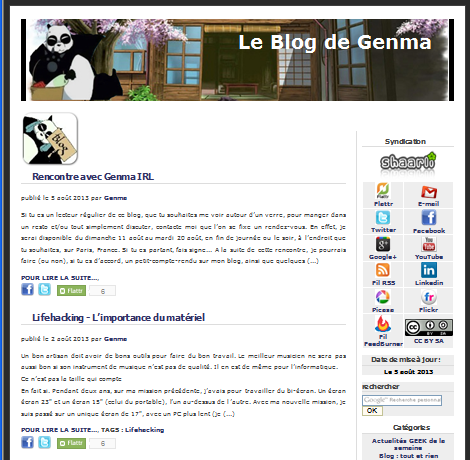
\includegraphics[width=5cm,height=5cm]{./materials/blog.png} 
\end{columns}
\end{frame}


%----------------------------------------------------------------------------------------
\begin{frame}
\frametitle{Digital identity, what is it?}

\begin{block}{Definition}
\begin{itemize}
\justifying{
\item Digital identity is all the public data you can find about someone using Internet research.
\item It's the famous e-reputation.
}
\end{itemize}
\end{block}
\begin{center}

\includegraphics[scale=0.5] {./materials/On-The-Internet-Nobody-Knows-Youre-A-Dog.jpg}
\end{center}

\end{frame}

%----------------------------------------------------------------------------------------
\begin{frame}
\frametitle{What do you think of me?}

\justifying{
\begin{block}{Google you name}
\begin{itemize}
\item The results shown are they exactly what you want?
\end{itemize}
\end{block}
}
\begin{center}
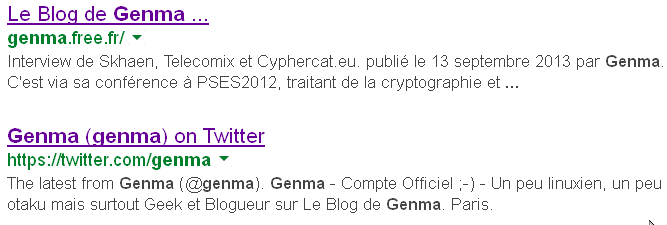
\includegraphics[scale=0.3] {./materials/Google01.png}
\\
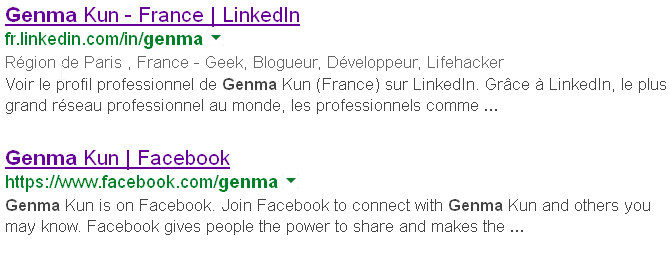
\includegraphics[scale=0.3] {./materials/Google02.png}
\end{center}
\end{frame}

%----------------------------------------------------------------------------------------
\begin{frame}
\frametitle{Saying}

\begin{block}{Words fly, writings remain}
\begin{itemize}
\justifying{
\item This adage is especially true with the Internet.
\item It must be assumed that what is said will always be accessible, even years later.
\item Everything on the Internet is public or will be (even if it is "private", Terms of Use may change).
\item It is therefore not abuse the freedom of expression and remain respectful of laws.
}
\end{itemize}
\end{block}


\end{frame}

%----------------------------------------------------------------------------------------
\begin{frame}
\frametitle{Pseudonymity}


\begin{block}{Defintion}
\begin{itemize}
\justifying{
\item Contraction of anonymity and pseudonym words, the term pseudonymity reflects quite well the contradictory of \textbf{being a public figure and to remain anonymous} ...
\item Have a pseudonym does not mean to say and do anything.
\item This is the image that I return, this is my credibility (past, present and future).
\item A pseudonym is also a public identity, which is associated with different account: my blog, my Twitter, my Facebook account.
\item The digital identity are all these public data associated with this identity.
}
\end{itemize}
\end{block}

\end{frame}


%----------------------------------------------------------------------------------------
\begin{frame}
\frametitle{Samples}

\begin{block}{Twitter}
\begin{center}
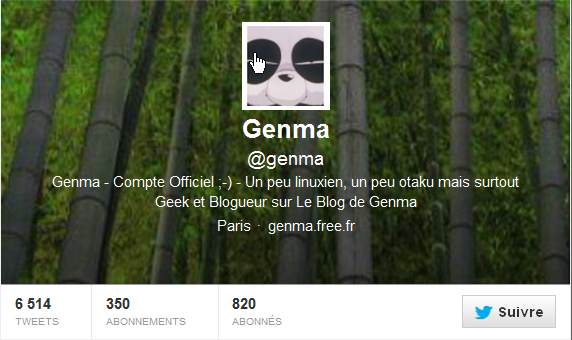
\includegraphics[scale=0.2] {./materials/Twitter.png}
\end{center}
\end{block}

\begin{block}{Linkedin}
\begin{center}
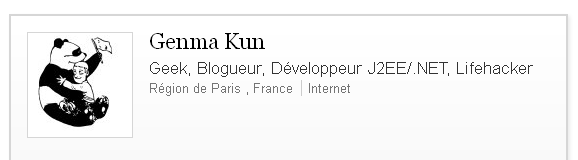
\includegraphics[scale=0.3] {./materials/Linkedin.png}
\end{center}
\end{block}
\end{frame}


%----------------------------------------------------------------------------------------
\begin{frame}
\frametitle{Pseudonymity is disapearing...}

\justifying{
\begin{block}{Facebook}
\begin{itemize}
\item Facebook doesn't allow the creation an account with a pseudonym,
    if you really want there is some easy steps to follow.
\item The goal is to force people to express themselves using their real names,
\end{itemize}
\end{block}
}

\end{frame}

%----------------------------------------------------------------------------------------
\begin{frame}
\frametitle{Pseudonymity is seen as a problem}

\justifying{
The problem is that the anonymity is take as an excuse to condemn the use of the Internet as a tool for freedom of expression. 
\\
If people are monitored, they do not say what they think, they do not criticize the politicians. 
\\
With the Internet, the citizen is gradually taking power on politicians.
}

\end{frame}

%----------------------------------------------------------------------------------------
\begin{frame}
\frametitle{Conclusion}
\justifying{
\begin{block}{Pseudonymity is a necessity}
\begin{itemize}
\item Manage your digital identity.
\item \textbf{Pseudonymity is the first step to take back you privacy.}
\end{itemize}
\end{block}
}

\end{frame}

 %--Genma
%--------------------------------------------------
\begin{frame}
\frametitle{Something unclear ?}
\begin{columns}[c]
\column{.5\textwidth}
\begin{figure}

\includegraphics[width=0.8\linewidth]{./materials/questions.jpg}
\end{figure}
\column{.5\textwidth}
Feel free to ask for questions now.
\end{columns}
\end{frame}



%---------------------------------------------------
\section{HOW TO: Encryption}
\subsection{WTF is encryption?}
%------------------------------------------------
\begin{frame}
\frametitle{Definition - cryptage, encrypt, encryption ?}

\begin{block}{Encryption}
\justifying{
Encryption is to encrypt a document / file using an encryption key.
The reverse operation is decryption.
}
\end{block}
\begin{block}{Cryptage}
\justifying{
Term « cryptage » is derived from the English encryption and does not exist in French.
Decryption is the fact of breaking the encryption when the private key is unknown.
}
\end{block}
\begin{block}{Cryptography}
\justifying{
Science is called Cryptography.
}
\end{block}
\end{frame}

%------------------------------------------------
\begin{frame}
\frametitle{Encryption, how does it work?}

\begin{block}{Symetric Encryption}
\justifying{
This involves encrypting a message with the same key that will be used for decryption process.
\\
Sample : Caesar code,  with an offset letter. A->C, B->D etc.
\\
Nous venons en paix ->  Pqwu xgpqpu gp rckz
\\
The reverse process is applied to get the message.
}
\end{block}

\begin{block}{What is an encryption key?}
\justifying{

A key is called so because it opens / closes the padlock that is the used encryption algorithm.
\begin {itemize}
\item Here, the algorithm is the offset.
\item The key is the number of offset of letter (here two letters).
\end{itemize}
}
\end{block}

\end{frame}

%------------------------------------------------
\begin{frame}
\frametitle{Asymetric Encryption 1/2}

\begin{block}{Public key - Private key}
\justifying{

Asymetric Encryption is based on the pair public key - private key.
\\$\Rightarrow$ What you need to know: 
\begin{itemize}
\item My private key is... private and my own.
\item My public key is shared with everyone.
\end{itemize}
}
\end{block}
	
\begin{block}{The encryption algorithm}
\justifying{
The encryption algorithm is more complexe than the fact of shifting letters ; it is based on mathematical concepts (first number ...)
}
\end{block}

\end{frame}

\begin{frame}
\frametitle{Asymetric Encryption 2/2}

\begin{block}{Encryption}
With the public key of my correspondent, I encrypt a file.
\justifying{
\\$\Rightarrow$ The file can only be decrypted by the person who possesses the private key corresponding to the public key that I used (and therefore my correspondent).
}
\end{block}

\begin{block}{Decryption}
With its private key, my correspondent decrypts the file.
\\
$\Rightarrow$ He can then read the message.
\end{block}

\begin{block}{Concret case}
Mail Encryption with PGP.
\end{block}
\end{frame}

%----------------------------------------------------------------------------------------
\begin{frame}
\frametitle{Bob send a message to Alice}
\begin{center}
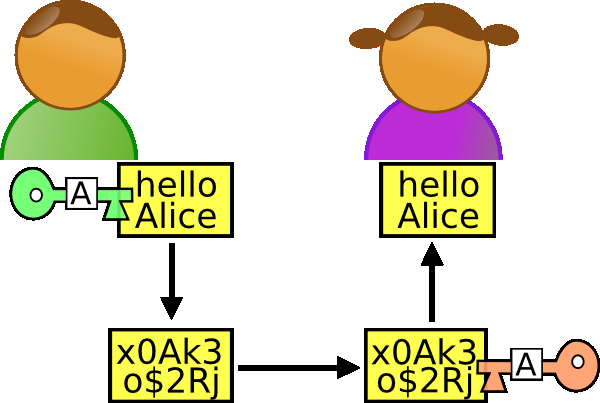
\includegraphics[scale=0.3] {./materials/Alice_et_bob} 
\end{center}
\end{frame}


%----------------------------------------------------------------------------------------
\begin{frame}
\Huge{\centerline{Why encryption?}}
\begin{center}
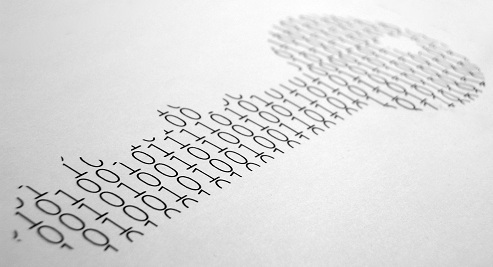
\includegraphics[scale=0.4] {./materials/cryptography.jpg} 
\end{center}
\end{frame}

%------------------------------------------------
\begin{frame}
\frametitle{Encrypt - The arguments against}

\justifying{
\begin{block}{Nobody does...}
FALSE. Without knowing it, you do it every day.
\\
Sample 1: "padlock" when connecting (https)
\\ Sample 2: Wifi key.
\end{block}

\begin{block}{Nothing to hide...}
FALSE. Who would accept the postman read his medical post ?
\end{block}

\begin{block}{Encryption, it's for the pedo-nazi...}
\justifying{
FALSE. For journalists / bloggers dissidents who are denouncing dictatorships...
}
\end{block}
}
\end{frame}

%------------------------------------------------
\begin{frame}
\frametitle{Encrypt - The arguments for}

\begin{block}{Encryption, it's not so complicated}
It is not more complicated than using a "software". You just have to understand the principle.
\end{block}

\begin{block}{Protection and security}
My personnal data are safe Cf. PRISM, NSA...
\end{block}

\begin{block}{Privacy}
Only the person for who the "message" is, is able to read it.
\end{block}

\end{frame}

%----------------------------------------------------------------------------------------
\begin{frame}
\frametitle{Edward Snowden}
\justifying{
Encryption works. Properly implemented strong crypto systems are one of the few things that you can rely on.
}
\begin{center}
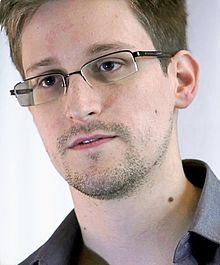
\includegraphics[scale=0.4] {./materials/snowden.jpg} 
\end{center}

\end{frame}


%------------------------------------------------
\begin{frame}
\frametitle{Encryption limit}
\begin{block}{Which is encrypted can be decrypted today tomorrow}
\justifying{
Tomorrow's computers will allow to decrypt the encrypted data today.
}
\end{block}

\begin{block}{It the private key is lost}
We no longer have access to data.
\end{block}

\begin{block}{Metadata, social graph}
\justifying{
\textbf{PGP does not protect against the analysis of metadata (servers transit, addresses, headers, subject).}
Do not forget to clean the meta-data files (EXIF tag photos, office documents with tracked changes).
DNS... Case of tracking Internet ...}
\end{block}

\end{frame}

%----------------------------------------------------------------------------------------
\begin{frame}
\frametitle{Law and encryption}
\justifying{
In France, the law therefore considers that the use of cryptology is free (LCEN Article 30-1) and there is therefore now no limit to the size of the encryption key that can be used .
\\~\\
In case of search, the refusal of submission of the encryption key may result in 3 years imprisonment and 45000\euro{}.
\\~\\
This penalty is increased if Encryption was used to commit a crime.
\\~\\
It is therefore recommended to give the decryption key, except in the case where the decrypted data would result in a judicial proceeding in which the final sentence would be greater than the interference with the judicial investigation.
}
\end{frame}

 %--Genma
\subsection{What can I encrypt? How?}
%------------------------------------------------
\begin{frame}
\frametitle{Le chiffrement}
\justifying{
\begin{block}{En local - ses données}
\begin{itemize}
\item Son disque dur
\item Sa clef USB
\item Son smartphone
\end{itemize}
\end{block}

\begin{block}{En réseau - ses communications}
\begin{itemize}
\item Https : utilisation de l'extension HTTPSEveryWhere pour Firefox  
\item Ses e-mails : utilisation de GPG via Enigmail pour Thunderbird
\item Sa connexion : utiliser un VPN, SSH, la clef "WIFI".
\end{itemize}
\end{block}

\begin{block}{}
$\Rightarrow$ \`A chaque "usage", il y a une solution de chiffrement possible.
\end{block}
}
\end{frame}


%----------------------------------------------------------------------------------------
\begin{frame}
\frametitle{Les mails - PGP, GPG?}
\begin{block}{PGP}
\justifying{
Pretty Good Privacy - PGP est un logiciel de chiffrement et de déchiffrement cryptographique, créé par l'américain Phil Zimmermann en 1991.
}
\end{block}
\begin{block}{OpenPGP}
\justifying{
Ce standard décrit le format des messages, signatures ou certificats que peuvent s'envoyer des logiciels comme GNU Privacy Guard. Ce n'est donc pas un logiciel, mais un format pour l'échange sécurisé de données, qui doit son nom au programme historique Pretty Good Privacy (PGP).
}
\end{block}
\begin{block}{GnuPG}
\justifying{GnuPG (ou GPG, de l'anglais GNU Privacy Guard) est l'implémentation GNU du standard OpenPGP.}
\end{block}
\end{frame}


%----------------------------------------------------------------------------------------
\begin{frame}

\frametitle{Chiffrer son disque dur}
\begin{block}{Logiciels intégrés aux systèmes d'exploitations}
\begin{itemize}
\item Windows 7/8 : Bitlocker (Backdor)
\item MacOS : FileVault
\item GNU/Linux : Encfs...
\end{itemize}
Peut-on faire confiance à autre chose que du logiciel libre ?
\end{block}

\begin{block}{Indépendament du système d'exploitation}
$\Rightarrow$ Le logiciel TrueCrypt. Pour une clef USB/un disque dur externe.
\end{block}
\end{frame}

%----------------------------------------------------------------------------------------
\begin{frame}
\frametitle{L'audit de TrueCrypt}
\begin{center}
 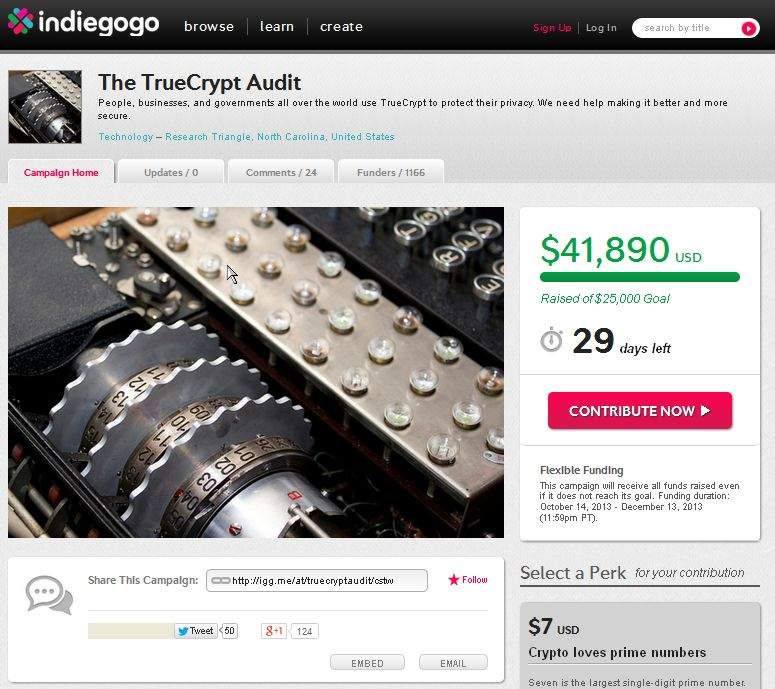
\includegraphics[scale=0.45] {./materials/truecryptaudit.jpg} 
\end{center}
\end{frame}
 %--Genma
%--------------------------------------------------
\begin{frame}
\frametitle{Encryption for connexions : SSL/TLS}
\begin{itemize}
\item Session layer based, affect application layer (TFP, HTTP, SMTP, IMAP, POP
, DNS, RTMP ...)
\item Prefer using TLS over SSL when you have choice.
\item Asymetrical encryption, forward secrecy (Diffie-Hellman).
\end{itemize}

Only use up to date browser in order to have the correct fingerprint cached
on your computer and avoid MITM attack.
If your browser does not have a certificate pinning system install
certificate patrol (assuming your first connection is safe) or HTTPS everywhere
with the SSL observatory ON.
\end{frame}

\begin{frame}
\frametitle{Diffie-Hellman key exchange}
\begin{columns}[c]
\column{.6\textwidth}
\begin{block}{With color}
\begin{itemize}
\item two person that never met agrees on the same keys
\item heavy use of one-way function
\item Select a public color, then each part select a private secret one.
\item each part mix private/public key and send it to the other.
\item Each part mix the mixture of the other with their own private color and
arrive to the same final private color.
\end{itemize}
\end{block}
\column{.4\textwidth}
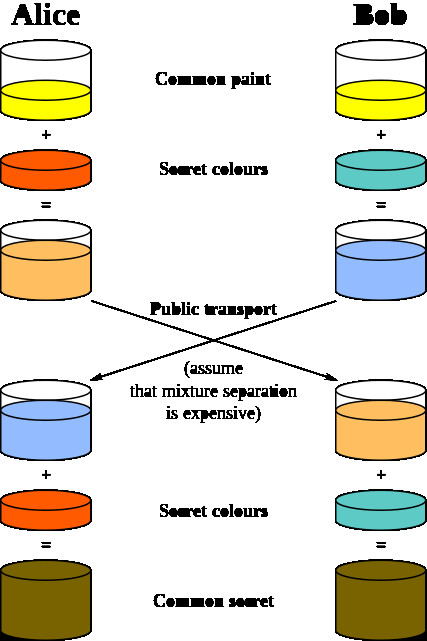
\includegraphics[height=.8\textheight]{./materials/diffie-hellman}
\end{columns}
\end{frame}
%----------------------------------------------------
\begin{frame}
\frametitle{Diffie-Hellman key exchange}
\begin{columns}[c]
\column{.6\textwidth}
\begin{block}{With maths : (modular|clock) arithmetic}
\begin{itemize}
\item work on prime modulus and generator of that modulus.
\item $3^n mod 17 = X$ with $0 <= X <= 17$ hard to reverse when len(prime modulus)
increase.
\item so each part agree on a prime modulus (p) and a generator (g).
Then calculate $g^{secret} mod(p)=Mix$ and send it publicly.
\item each part compute now $Mix^{secret} mod(p)=Key$
\end{itemize}
\end{block}
\column{.4\textwidth}
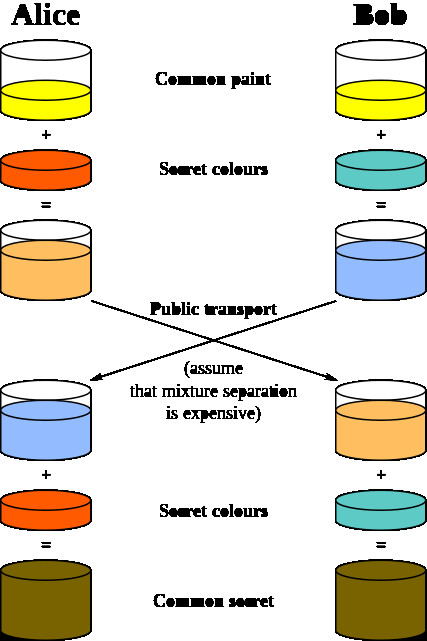
\includegraphics[height=.8\textheight]{./materials/diffie-hellman}
\end{columns}
\end{frame}
%--------------------------------------------------
\begin{frame}
\frametitle{Encryption for chat sessions : OTR}
\begin{block}{OTR : Off-the-Record Messaging}
\begin{itemize}
\item Diffie-Hellman key exchange
\item off-the-record conversation
\item repudiable authentication by using message authentication codes.
\\(authentication ON | digital signature OFF)
\end{itemize}
\end{block}
Bob cannot prove that Alice generated the MAC.
Install Pidgin (cross-plateform) with plugin (available from the OTR homepage)
and start playing.
\end{frame}
%----------------------------------------------------
\begin{frame}
\frametitle{Encryption for disk}
Many possibilities, but full disk encryption is advised in case you really care
about privacy. For this purpose you have a plethora of choice.
\begin{itemize}
\item Stacked filesystem encryption (eCryptfs, EncFs, disk utility ...)
\item Disk encryption (dm-crypt, GELI, FileVault, DiskCryptor, trueCrypt ...)
\end{itemize}
\begin{block}{Case study : Plain dm-crypt}
\begin{itemize}
\item full disk encryption
\item bootloader and key on external device
\end{itemize}
\end{block}
(can also be done with Diskcryptor)
\end{frame}
%----------------------------------------------------
\begin{frame}
\frametitle{Encryption for smartphone}
\begin{block}{Android}
\begin{itemize}
\item Chatsecure (Facebook chat, GTalk, Jabber) [OTR Messaging]
\item Textsecure (SMS)
\item LUKS Manager (ROOT requiered)
\end{itemize}
\end{block}
\begin{block}{iOS}
\begin{itemize}
\item Chatsecure (Facebook chat, GTalk, Jabber) [OTR Messaging]
\item FDE available by default, bypass techniques available, proprietary
built system...\\ (More details : iPhone Forensic, O'Reilly)
\end{itemize}
\end{block}
\end{frame}
%----------------------------------------------------
\begin{frame}
\frametitle{Example chatsecure with facebook}
TODO
\end{frame}
%----------------------------------------------------
\begin{frame}
\frametitle{Encryption for files}
\begin{block}{Mails : Use GPG}
\begin{itemize}
\item create your keys
\item share your public key
\item enter the \sout{matrix} Web Of Trust (WOT)
\item encrypt/sign your message and send it.
\item receive mails too.
\end{itemize}
\end{block}
\begin{block}{Files}
Basically you can do the same with 'regular file'...
Take care to not store keys near encrypted files, prefer symetrical encryption
if files will not be shared.
\end{block}
\end{frame}

%----------------------------------------------------
\begin{frame}
\frametitle{Choosing a password : Diceware method}
The diceware method allow you to construct very strength password with the
following adventages :
\begin{itemize}
\item Very easy to remember
\item strong passphrase with high entropy (~20char +)
\item trully random; password is totally detached from user habits/knowledge
etc.
\end{itemize}
\begin{block}{Test your password strength in bits}
Entropy calculated by : $H_{tn}=\sum_{k=1}^nL*\frac{Log N}{Log 2}$
\end{block}
Do \emph{NOT} test your password strength online.
Take a calculator and calcul the entropy yourself.
\end{frame}
%----------------------------------------------------
\begin{frame}
\frametitle{Diceware, overall strength}
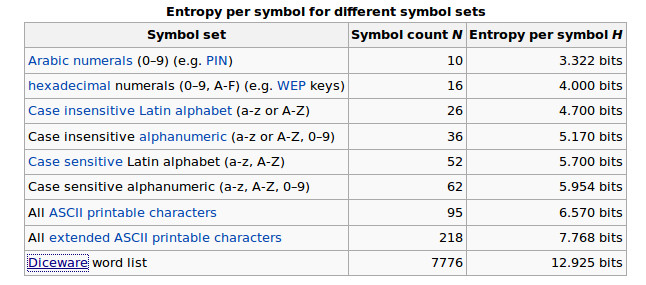
\includegraphics[width=0.8\linewidth]{./materials/diceware}
\end{frame}
%----------------------------------------------------
\begin{frame}
\frametitle{Diceware, how does it work}
You only need a true random source and an official mapped dictionary. \\
\begin{columns}[c]
\column{.5\textwidth}
\begin{itemize}
\item Draw 1 : 5 1 5 5 5
\item Draw 2 : 5 4 5 6 6
\item Draw 3 : 6 5 6 4 6
\item Draw 4 : 5 4 3 1 2
\item Draw 5 : 2 2 3 5 4
\end{itemize}
\column{.5\textwidth}
\begin{itemize}
\item ...
\item 14245 bit
\item 14246 bitch
\item 14247 bite
\item ...
\end{itemize}
\end{columns}
\begin{block}{Results}
\begin{itemize}
\item in French : phase ribose vv rebut clebs
\item in English : rest sober 80 skye data
\end{itemize}
\end{block}
\end{frame}
 %--Naam
%--------------------------------------------------
\begin{frame}
\frametitle{Something unclear ?}
\begin{columns}[c]
\column{.5\textwidth}
\begin{figure}

\includegraphics[width=0.8\linewidth]{./materials/questions.jpg}
\end{figure}
\column{.5\textwidth}
Feel free to ask for questions now.
\end{columns}
\end{frame}



%--------------------------------------------------
\section{HOW TO: Anonymity}
\subsection{Why does it matter?}
\begin{frame}
\begin{center}
\huge{Anonymity}
\end{center}
\begin{center}

\includegraphics[scale=0.5] {./materials/anonymity1.jpg} 
\end{center}
\end{frame}


\begin{frame}
\frametitle{Anonymity, why does it matter?}
\justifying{
In real life, anonymity is necessary for democraty (voting paper).
\\
On line, anonymity is necessary for freedom of expression.
}
\begin{center}

\includegraphics[scale=0.45] {./materials/vie_privee.jpg} 
\end{center}
\end{frame}
 %--Genma
\subsection{There is always a tool that fit your need}
%----------------------------------------------------------------------------------------
\begin{frame}
\begin{center}
\frametitle{Onion routing principles}
TODO: schema explicatif
\end{center}
\end{frame}


%---------------------------------------------------
\begin{frame}
\frametitle{TOR : The Onion Router}
It's an open-source implementation of the principles we just saw supported by
The Tor Project.
\begin{figure}

\includegraphics[width=0.5\linewidth]{./materials/septical_boy}
\end{figure}
\end{frame}
%---------------------------------------------------
\begin{frame}
\frametitle{TOR : The Onion Router}
\begin{block}{Pros}
\begin{itemize}
\item Hide you identity and location, prevents from eyesdropping.
\item Hide you browsing habbits and act like a debrider on the informations that
you're authorized to see.
\item encrypt your (incom|outgo)ing traffic between nodes.
\end{itemize}
\end{block}
\begin{block}{Cons}
\begin{itemize}
\item Slower connexion, forget about downloading big files, torrents
(deanonymize effect) etc...
\item Still vulnerable to some kind of analysis
\\ (timing deduction or infection between applications).
\item entry/exit nodes are vulnerables, no magic here.
\\ (Partial solution if you setup an exit enclaving node)
\end{itemize}
\end{block}
TOR is an anonymity tool, not a security one.
\end{frame}

%---------------------------------------------------
\begin{frame}
\frametitle{If you use it, do it smartly}
\begin{columns}[c]
\column{.5\textwidth}
\begin{itemize}
\item don't use standalone TOR or Vidalia bundlle
\item prefer the use of the TBB (Tor Browser Bundle)
\item or even better : tails (live Debian), in hostile environment
(public places etc)
\end{itemize}
\column{.5\textwidth}
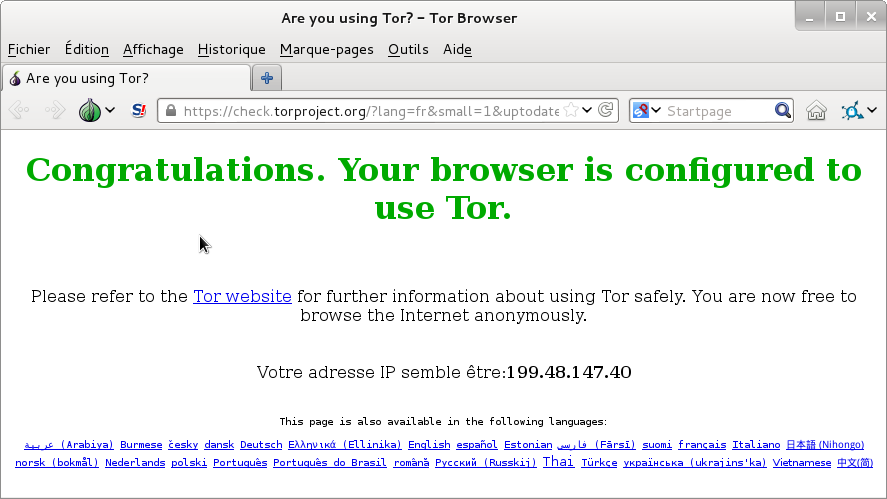
\includegraphics[keepaspectratio,width=\textwidth, height=.8\textheight]{./materials/tbb}
\end{columns}
Try Tor browser launcher for your distribution, that keep TBB updated. Grab-it
from here :\\ https://github.com/micahflee/torbrowser-launcher
\end{frame}
%----------------------------------------------------------------------------------------
\begin{frame}
\frametitle{Want to help ?}
give all your money to NosOignons.net (https://nos-oignons.net)
\end{frame}

%----------------------------------------------------------------------------------------
\begin{frame}
\begin{center}
\Huge{Sur Internet, si c'est gratuit, c'est vous le produit }
\end{center}
\end{frame}


%----------------------------------------------------------------------------------------
\begin{frame}
\frametitle{Qu'est-ce que le pistage ?}


\begin{block}{Le pistage sur Internet}
\begin{itemize}
\justifying{
\item Le pistage est un terme qui comprend des méthodes aussi nombreuses et variées que les sites web, les annonceurs et d'autres utilisent pour connaître vos habitudes de navigation sur le Web. 
\item  Cela comprend des informations sur les sites que vous visitez, les choses que vous aimez, n'aimez pas et achetez. 
\item Ils utilisent souvent ces données pour afficher des pubs, des produits ou services spécialement ciblés pour vous. 
}
\end{itemize}
\end{block}
\end{frame}


%----------------------------------------------------------------------------------------
\begin{frame}
\frametitle{Comment est-on tracké?}

\justifying{
\begin{block}{Toutes les publicités nous espionnent}
\begin{itemize}
\item Le bouton Like de Facebook : il permet à FaceBook de savoir que vous avez visité ce site, même si vous n'avez pas cliqué sur ce bouton.
\item Même si vous vous êtes correctement déconnecté de Facebook.
\item De même pour le bouton le +1 de Google, les scripts de Google Analytics, 
\item Tous les publicité, Amazon...
\end{itemize}
\end{block}
}
\begin{center}

\includegraphics[scale=0.3] {./materials/Facebook_like.png}
\end{center}
\end{frame}


%----------------------------------------------------------------------------------------
\begin{frame}
\frametitle{L'extension Firefox LightBeam (ex Collusion)}
Cette extension permet de voir en temps réel qui nous traque et les interconnexions qu'a le site actuellement visité avec d'autres sites.
\begin{center}
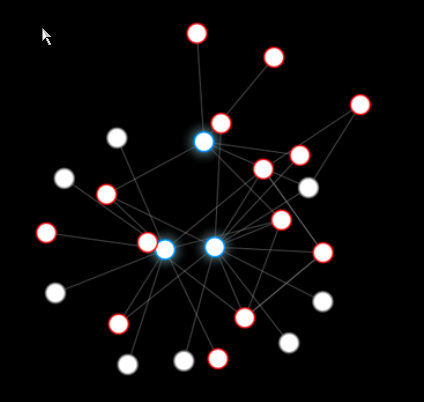
\includegraphics[scale=0.3] {./materials/Collusion.png}
\end{center}
\end{frame}

%----------------------------------------------------------------------------------------
\begin{frame}
\begin{center}
\Huge{Anomymat et extensions pour Firefox}
\end{center}
\end{frame}


%----------------------------------------------------------------------------------------
\begin{frame}
\frametitle{Noscript}

Bloque tous les trackers associés au site.

\begin{center}

\end{center}
\end{frame}


%----------------------------------------------------------------------------------------
\begin{frame}
\frametitle{Self destructing cookie}

Suppression automatisée des cookies

\begin{center}
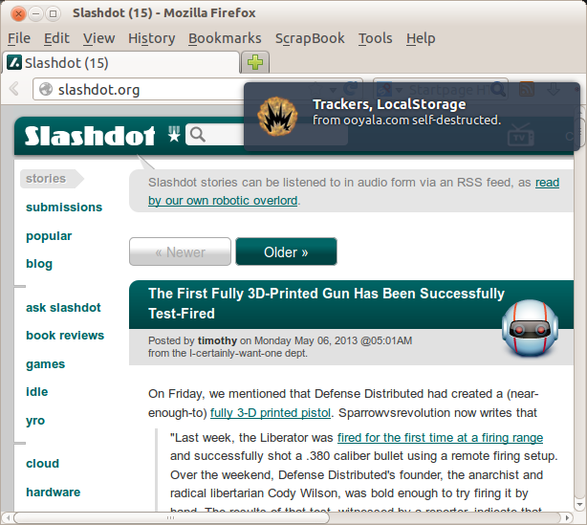
\includegraphics[scale=0.4] {./materials/selfdestructingcookie.png}
\end{center}
\end{frame}

%----------------------------------------------------------------------------------------
\begin{frame}
\begin{center}
\Huge{Changer de moteur de recherche}
\end{center}
\end{frame}

%----------------------------------------------------------------------------------------
\begin{frame}
\begin{center}
\frametitle{Duckduckgo - Google tracks you. We don't.}

\url{https://duckduckgo.com/}
\\

\includegraphics[scale=0.4] {./materials/DuckDuckGo.jpg}
\end{center}
\end{frame}

%----------------------------------------------------------------------------------------
\begin{frame}
\begin{center}
\Huge{Et pour plus de sécurité?}
\end{center}
\end{frame}

%----------------------------------------------------------------------------------------
\begin{frame}
\frametitle{HTTPSEverywhere}

Force le passage en https quand celui-ci est proposé par le site.

\begin{center}

\includegraphics[scale=0.4] {./materials/https-everywhere.jpg}
\end{center}

\end{frame}

%----------------------------------------------------------------------------------------
\begin{frame}
\frametitle{Certificate Patrol}
Permet de valider les certificats d'un site (lié à https).
\begin{center}
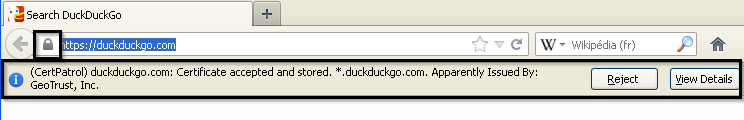
\includegraphics[scale=0.4] {./materials/CertificatePatrol.png}
\end{center}
\end{frame}

 %--Naam
%--------------------------------------------------
\begin{frame}
\frametitle{Something unclear ?}
\begin{columns}[c]
\column{.5\textwidth}
\begin{figure}

\includegraphics[width=0.8\linewidth]{./materials/questions.jpg}
\end{figure}
\column{.5\textwidth}
Feel free to ask for questions now.
\end{columns}
\end{frame}



%--------------------------------------------------
\section{Conclusion}
\subsection{We're not in a XOXO word}
\begin{frame}
\frametitle{Le crypto-anarchisme}
Tout le monde chiffre et ce qui est vraiment important est chiffré et noyé dans la masse.
\\~\\
On crée du bruit ce qui empêche la surveillance de masse (Affaire PRISM...)
\\~\\
Attention, à l'heure actuel, le chiffrement étant peu répandu, toute personne qui chiffre ses e-mails pourra être considérée comme suspecte.
\end{frame}


\begin{frame}
\frametitle{Relativité de l'anonymat de nos jours}

\justifying{
\begin{block}{Analyse sur les éléments de langage}
\begin{itemize}
\item On peut identifier quelqu'un à sa typographie, son style, son vocabulaire, sa culture, ses idées.. 
\item La fréquence des mots utilisés, la tournure de phrase, le genre...
\item Techniques utilisées pour déterminer qui se cachent derrière des Anonymous...
\end{itemize}
\end{block}
}

\justifying{
\begin{block}{Attention aux Logs}
\begin{itemize}
\item Les horaires de connexions et l'estimation du fuseau horaire donnent également des informations...
\end{itemize}
\end{block}
}

\end{frame}


\begin{frame}

\end{frame}

%----------------------------------------------------------------------------------------
\begin{frame}
\frametitle{Want to help ?}
give all your money to NosOignons.net (https://nos-oignons.net)
... TODO add others.
\end{frame}



%--------------------------------------------------

\subsection{Cryptoparty}
\begin{frame}
\end{frame}
 %--Naam
%--------------------------------------------------

%--------------------------------------------------
\begin{frame}
\frametitle{Something unclear ?}
\begin{columns}[c]
\column{.5\textwidth}
\begin{figure}

\includegraphics[width=0.8\linewidth]{./materials/questions.jpg}
\end{figure}
\column{.5\textwidth}
Feel free to ask for questions now.
\end{columns}
\end{frame}



%--------------------------------------------------
\begin{frame}
\frametitle{Rendez vous at the Cryptoparty}
\begin{figure}

\includegraphics[width=0.8\linewidth]{./materials/cryptoparty.jpg}
\end{figure}
\end{frame}
%--------------------------------------------------
\end{document}
